\documentclass[lang=cn,10pt,newtx]{elegantbook}
\usepackage{tikz}
\usepackage{float}
\newtheorem{Thm}{\hspace{2em}定理}[section]
\newcommand{\supp}{\text{supp}}
\newcommand{\dif}{\mathrm{d}}
\newcommand{\avg}[1]{\left\langle #1 \right\rangle}
\newcommand{\difFrac}[2]{\frac{\dif #1}{\dif #2}}
\newcommand{\pdfFrac}[2]{\frac{\partial #1}{\partial #2}}
\newcommand{\OFL}{\mathrm{OFL}}
\newcommand{\UFL}{\mathrm{UFL}}
\newcommand{\fl}{\mathrm{fl}}
\newcommand{\op}{\odot}
\newcommand{\cp}{\cdot}
\newcommand{\Eabs}{E_{\mathrm{abs}}}
\newcommand{\Erel}{E_{\mathrm{rel}}}
\newcommand{\DR}{\mathcal{D}_{\widetilde{LN}}^{n}}
\newcommand{\add}[2]{\sum_{#1=1}^{#2}}
\newcommand{\innerprod}[2]{\left<#1,#2\right>}
\newcommand{\norm}[1]{\|#1\|}
\newcommand\tbbint{{-\mkern -16mu\int}}
\newcommand\tbint{{\mathchar '26\mkern -14mu\int}}
\newcommand\dbbint{{-\mkern -19mu\int}}
\newcommand\dbint{{\mathchar '26\mkern -18mu\int}}
\newcommand\bint{
{\mathchoice{\dbint}{\tbint}{\tbint}{\tbint}}
}
\newcommand\bbint{
{\mathchoice{\dbbint}{\tbbint}{\tbbint}{\tbbint}}
}
\title{Note For Finite Element Methods}
\subtitle{Zhejiang University}

\author{Shuang Hu}
\institute{Zhejiang University}
\date{Sept 14, 2022}
\version{1.0}
\bioinfo{简介}{2022秋冬学季“有限元方法”课程笔记}

\setcounter{tocdepth}{3}

\logo{logo-blue.png}
\cover{cover.jpg}

% 本文档命令
\usepackage{array}
\newcommand{\ccr}[1]{\makecell{{\color{#1}\rule{1cm}{1cm}}}}

% 修改标题页的橙色带
\definecolor{customcolor}{RGB}{32,178,170}
\colorlet{coverlinecolor}{customcolor}
\usepackage{cprotect}

\addbibresource[location=local]{reference.bib} % 参考文献,不要删除

\begin{document}

\maketitle
\frontmatter

\tableofcontents

\mainmatter

\chapter{一维有限元方法}
\section{为什么需要有限元方法?}
此前在《微分方程数值解》课程中,我们已经学习了有限差分法和有限体积法。这两种方法有不少优点:首先,比较直观,只要知道如何利用差分近似导数即可得到对应的差分公式;其次,在一些情形下,有限差分和有限体积方法可以实现较高的计算精度。

但是,这两种算法有一些明显的缺陷。
\begin{itemize}
  \item 算法稳定性的分析比较复杂。
  \item 处理不规则区域的问题时较为麻烦,需要多次利用插值近似。
  \item 只是求解离散格点的近似点值/离散网格的近似积分平均值,未能给出函数整体的近似。
\end{itemize}

为此,基于函数逼近论的\textbf{有限元方法}被提出。该算法能弥补有限差分法的一些明显缺陷,目前是最主流的数值算法之一。
\section{从一维边值问题说起}
考虑如下例子:
\begin{equation}
  \label{eq:ode1}
  \left\{
    \begin{aligned}
    -u''+u&=f(x),x\in(0,1)\\
    u(0)=u(1)&=0.
    \end{aligned}
  \right.
\end{equation}
类似于“偏微分方程”课程中对弱解的讨论方式,在\eqref{eq:ode1}两边同时乘某个函数$v$并在$[0,1]$上积分,得到如下形式:
\begin{equation}
  \label{eq:bianfen}
  \int_{0}^{1}(-u''+u)v\dif x=\int_{0}^{1}fv\dif x.
\end{equation}
定义函数空间$V$如下:
\begin{equation}
  \label{eq:sobolev1-1}
  V:=\left\{v\left.\right|v(0)=v(1)=0,\int_{0}^{1}((v')^{2}+v^{2})\dif x<\infty\right\}.
\end{equation}
如果函数$v\in V$, 利用分部积分法,\eqref{eq:ode1}可以转化为以下问题:
\begin{example}
  \label{ex:equiv1}
  记$a(u,v)=\int_{0}^{1}(u'v'+uv)\dif x$, $h(v)=\int_{0}^{1}fv\dif x$, $v\in V$.求$u\in V$,使得$a(u,v)=h(v)$ $\forall v\in V$.
\end{example}
下面的定理说明了该问题可以转化为一个优化问题:
\begin{theorem}{}{}
  \label{thm:bianfen}
  记泛函$J(v):=\frac{1}{2}a(v,v)-h(v)$,问题\ref{ex:equiv1}与最小化$J(v)$的优化问题等价。即:如果$a(u,v)=h(v)\forall v\in V$, 那么$J(u)\le J(v)\forall v\in V$。
\end{theorem}
\begin{proof}
  $\Rightarrow$:
  \begin{equation}
    \label{eq:dif}
    \begin{aligned}
      J(v)-J(u)&=\frac{1}{2}a(v,v)-h(v)-\frac{1}{2}a(u,u)+h(u)\\
      &=\frac{1}{2}(a(v,v)-a(u,u)-2h(v-u))\\
      &=\frac{1}{2}(a(v,v)-a(u,u)-2a(u,v-u))\\
      &=\frac{1}{2}(a(v,v)+a(u,u)-2a(v,u))\\
      &=\frac{1}{2}(a(v-u,v-u))\ge0.
    \end{aligned}
  \end{equation}
  由\eqref{eq:dif}可得,如果$a(u,v)=h(v)$,那么$J(u)\le J(v)$.

  $\Leftarrow$: $\forall v\in V$, $t\in\mathbb{R}$,有$J(u+tv)\ge J(u)$。我们定义函数$g(t):=J(u+tv)$,根据上面的讨论可知:$g'(0)=0$。另一方面,计算$g(t)$的表达式,有:
  \begin{equation}
    \begin{aligned}
      \label{eq:gt}
      g(t)&=J(u+tv)\\
      &=\frac{1}{2}\int_{0}^{1}((u'+tv'
      )^{2}+(u+tv)^{2})\dif x-\int_{0}^{1}f(u+tv)\dif x\\
    \end{aligned}
  \end{equation}
  对\eqref{eq:gt}求一阶导数,可得:
  \begin{equation}
    \label{eq:dirg0}
    g'(0)=\int_{0}^{1}(u'v'+uv)\dif x-\int_{0}^{1}fv\dif x.
  \end{equation}
  根据$g$的一阶条件,可得$a(u,v)=h(v)$。又由于$v$的任意性,结论得证。
\end{proof}

如此,我们把一个解微分方程的问题,利用\ref{ex:equiv1}和\ref{thm:bianfen}转化为了一个变分问题。由于$V$是一个无穷维空间,我们不能期望利用算法给出这个变分问题的精确解,但我们可以考虑对空间$V$进行有限维近似,并在有限维空间上近似求解这个变分问题。

\section{有限元思想的导出}
接下来,根据上一节的思路,我们继续问题\eqref{eq:ode1}的近似求解。根据上面的分析,我们的数值算法需要解决两个问题:
\begin{itemize}
  \item 如何对函数空间$V$进行有限维近似?
  \item 在进行有限维近似之后,如何在有限维空间中对变分问题进行求解?
\end{itemize}
首先,我们考虑第二个问题。根据上面的讨论,近似求解变分问题有两种不同的思路,分别对应的是\textbf{Galerkin近似方法}和\textbf{Ritz近似方法}。
\subsection{Galerkin近似}
\textbf{假设已经给出有限维子空间}$V_{N}\le V$,Galerkin近似的目的是求解$u_{N}\in V_{N}$使得
\begin{equation}
  \label{eq:Galerkin}
  a(u_{N},v_{N})=h(v_{N})
\end{equation}
对所有$v_{N}\in V_{N}$都成立。

由于$V_{N}$是有限维的空间,我们可以找到这个空间中的一组基函数$\{\phi_{1},\cdots,\phi_{N}\}$,注意到$a(u,v)$是对称双线性函数,设$u_{N}=\alpha_{1}\phi_{1}(x)+\cdots+\alpha_{N}\phi_{N}(x)$,$v_{N}(x)=\phi_{i}(x)$,代入\eqref{eq:Galerkin},可得一个线性方程组:
\begin{equation}
  \label{eq:LinearSystem}
  \begin{bmatrix}
    a(\phi_{1},\phi_{1})&a(\phi_{1},\phi_{2})&\cdots&a(\phi_{1},\phi_{N})\\
    a(\phi_{2},\phi_{1})&a(\phi_{2},\phi_{2})&\cdots&a(\phi_{2},\phi_{N})\\
    \vdots&\vdots&\ddots&\vdots\\
    a(\phi_{N},\phi_{1})&a(\phi_{N},\phi_{2})&\cdots&a(\phi_{N},\phi_{N})\\
  \end{bmatrix}
  \begin{bmatrix}
    \alpha_{1}\\
    \alpha_{2}\\
    \vdots\\
    \alpha_{N}\\
  \end{bmatrix}
  =\begin{bmatrix}
    h(\phi_{1})\\
    h(\phi_{2})\\
    \vdots\\
    h(\phi_{N})\\
  \end{bmatrix}
\end{equation}
解这个线性方程组,得到系数向量,即可给出该方程的近似解。

\subsection{Ritz方法}
同样,假设有限维子空间$V_{N}\le V$已经给出,\textbf{Ritz方法}的思路是求解有关$J(u)$的优化问题,即:求$u_{N}\in V_{N}$,使得
\begin{equation}
J(u_{N})\le J(v)\forall v\in V_{N}.
\end{equation}
这里$J(v):=\frac{1}{2}a(v,v)-h(v)$。

给出这个问题之后,我们在有限维空间中,利用最优化算法求解该问题。

这两个思路都是建立在有限维子空间$V_{N}$已经给出的前提下的。但这个有限维空间如何构造?

一个很容易想到的思路是利用$v(0)=v(1)$这一性质,构造三角函数系作为基底。这种选取思路对于问题\eqref{eq:ode1}而言当然是极好的,三角函数系的正交性也使得\eqref{eq:LinearSystem}中的系数矩阵变得相当简单易求解。但这个方案的可扩展性并不强,如果扩展到二维平面上,乃至更高维度的椭圆偏微分方程,就很难找到像这样全局定义的基函数。如果问题区域非规则或是存在不同方程的耦合,则更是如此。

\textbf{有限元方法}由此引出。
\section{有限元方法}
在上面两种思路的基础上,我们需要一个方便推广的构建有限维子空间的方法。

多项式函数空间是最容易表示的函数空间,因此这是我们的首选。但全局定义的多项式很难保证其符合边界条件。于是,借助样条插值的思想,我们转为考虑分段多项式空间。

\subsection{线性有限元空间}
我们先针对问题\eqref{eq:ode1},考虑最简单的近似形式--分段线性近似。在这种情形下,有限维子空间$V_{h}$由$(0,1)$上的分段线性函数表示。
\begin{definition}{线性有限元空间}
  \label{LinearFE}
  线性有限元空间的定义为:
  \begin{equation}
    \label{eq:linearFE}
    V_{h}:=\{v_{h}\in C(0,1):v_{h}(0)=v_{h}(1)=0,v_{h}|_{[x_{i},x_{i+1}]}\in\mathbb{P}_{1}\}.
  \end{equation}
  其中$\{x_{i}\}_{i=0}^{n}$为$[0,1]$上给定的互异节点,$x_{0}=0$,$x_{n}=1$。
\end{definition}
首先需要讨论的是,空间$V_{h}$的维数和基底。空间\eqref{eq:linearFE}的形式很容易联想到数值分析课程中学习过的\textbf{B-样条空间}。特别地,一维B-样条基函数为所谓的“hat-function”,定义如下:
\begin{equation}
  \label{eq:hatfunc}
  \phi_{i}(x)=\left\{
    \begin{aligned}
      &\frac{x-x_{i-1}}{x_{i}-x_{i-1}},x_{i-1}\le x\le x_{i}\\
      &\frac{x_{i+1}-x}{x_{i+1}-x_{i}},x_{i}\le x\le x_{i+1}\\
      & 0,otherwise\\
    \end{aligned}
  \right.
\end{equation}
\begin{figure}[H]
  \centering
  \caption{hat函数的示意图}
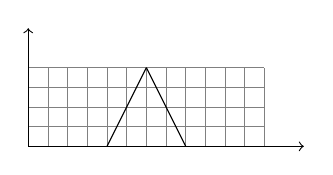
\begin{tikzpicture}
  \draw[step=.25cm,gray,very thin] (0,0) grid (3,1); 
  \draw [->](0,0) -- (3.5,0); 
  \draw [->](0,0) -- (0,1.5); 
  \draw (1,0) -- (1.5,1);
  \draw (1.5,1) -- (2,0);
\end{tikzpicture}
\end{figure}
容易验证,如此定义的$(\phi_{1},\cdots,\phi_{n-1})$构成了空间$V_{h}$的一组基。从而可得$\dim(V_{h})=n-1$。
\subsection{刚度矩阵与负载}
此处我们采用Galerkin近似的思路,下面我们需要讨论的是方程组\eqref{eq:LinearSystem}的导出与求解。

\begin{definition}{刚度矩阵}
  线性有限元空间\ref{LinearFE}的刚度矩阵定义为:
  \begin{equation}
    \label{eq:stablemat}
    A=(a(\phi_{i},\phi_{j}))_{i,j=1}^{n-1}.
  \end{equation}
  其中$\phi_{i}$为\eqref{eq:hatfunc}中定义的基函数。
\end{definition}

\begin{definition}{负载}
  方程\eqref{eq:ode1}关于线性有限元空间\ref{LinearFE}的负载向量定义为:
  \begin{equation}
    \label{eq:overload}
    \mathbf{b}:=\left(\int_{0}^{1}f(x)\phi_{i}(x)\dif x\right)_{i=1}^{n-1}.
  \end{equation}
\end{definition}

下面讨论\eqref{eq:ode1}负载的计算。由于我们是用一次样条多项式近似真实解的,在选取数值积分公式的时候只需要使用一阶代数精度的公式即可不损失计算精度。因此此处采用复化梯形公式进行负载的近似计算。

记$h_{i}=x_{i}-x_{i-1}$,负载的近似计算公式如下:
\begin{equation}
  b_{i}=\int_{0}^{1}f(x)\phi_{i}(x)\dif x=\int_{x_{i-1}}^{x_{i+1}}f(x)\phi_{i}(x)\approx \frac{1}{2}(h_{i}+h_{i+1})f(x_{i}).
\end{equation}

对于刚度矩阵的计算,虽然基函数$\phi_{i}$在整个区间$(0,1)$上并不可导,但不可导点为零测集,不会对积分的计算产生影响。将基函数$\phi_{i}$的表达式代入刚度矩阵,计算得:
\begin{equation}
  \label{eq:stablematval}
  \left\{
    \begin{aligned}
      a_{ij}&=0,|i-j|>1\\
      a_{ii}&=\frac{1}{h_{i}}+\frac{1}{h_{i+1}}+\frac{1}{3}(h_{i}+h_{i+1})\\
      a_{i-1,i}&=-\frac{1}{h_{i}}+\frac{1}{6}h_{i}\\
      a_{i,i+1}&=-\frac{1}{h_{i+1}}+\frac{1}{6}h_{i+1}\\
    \end{aligned}
  \right.
\end{equation}
由\eqref{eq:stablematval}可知,刚度矩阵是一个三对角矩阵,因此如果采用传统的矩阵存储方式和求解方式可能会造成计算资源的浪费。下面给出一种采用“局部矩阵”的形式存储\eqref{eq:stablematval}的技巧。

记负载矩阵$A=\sum_{k=1}^{n}A^{(k)}$,其中$A^{(k)}:=(a_{ij}^{(k)})$,$a_{ij}^{(k)}:=\int_{x_{k-1}}^{x_{k}}[\phi_{i}'(x)\phi_{j}'(x)+\phi_{i}(x)\phi_{j}(x)]\dif x$,由定义可得,$a_{ij}^{(k)}$只在$i,j\in\{k-1,k\}$时取非零值。所以每个$A^{(k)}$都可以存储为一个$2\times 2$的矩阵,而整体的负载矩阵$A$可以视为把所有的$A^{(k)}$“装配”起来的结果。在求解最终的线性方程组的时候,由于矩阵$A$是一个三对角对称正定矩阵,我们可以采用一系列数值代数算法加速方程组的求解。
\section{误差分析}
在本节中我们针对求解\eqref{eq:ode1}的线性有限元近似算法进行误差分析。在叙述之前,为方便起见,先给出两个记号。

\begin{remark}
  $\norm{f}_{0}$:表示$L^{2}$范数, $\norm{f}_{0}:=\sqrt{\int_{0}^{1}f^{2}\dif x}$。$\norm{f}_{1}$:表示$W^{1,2}$范数,$\norm{f}_{1}:=\sqrt{\int_{0}^{1}((f')^{2}+f^{2})\dif x}$。
\end{remark}

回顾一下有限元逼近问题的提法:
\begin{example}
  \label{prob:FE problem}
记泛函$a(u,v)=\int_{0}^{1}(uv+u'v')\dif x$, $h(v)=\int_{0}^{1}fv\dif x$, $V=\{v(x):v(0)=v(1)=0,\int_{0}^{1}((v')^{2}+v^2)\dif x<\infty\}$, 原问题是求解$u\in V$使得$a(u,v)=h(v)\forall v\in V$, 而在线性有限元空间上的逼近问题则是,在线性有限元空间$V_{h}\le V$上求解$u_{h}\in V$使得$a(u_{h},v_{h})=h(v_{h})\forall v_{h}\in V_{h}$。
\end{example}

在进行讨论前,首先给出一个重要的引理。该引理保证了在$W^{1,2}$范数的意义下,$u_{h}\in V_{h}$是$u\in V$在子空间$V_{h}$下的最优逼近。
\begin{lemma}{Cea引理}
  \label{lem:cea}
  设$u$和$u_{h}$是\ref{prob:FE problem}的解,则有:
  \begin{equation}
    \label{eq:cea}
    \norm{u-u_{h}}_{1}\le\inf_{v_{h}\in V_{h}}\norm{u-v_{h}}_{1}.
  \end{equation}
\end{lemma}
\begin{proof}
  由于$u$满足:$\forall v\in V, a(u,v)=h(v)\Rightarrow\forall v_{h}\in V_{h},a(u,v_{h})=h(v_{h})$。又有:$u_{h}$满足$a(u_{h},v_{h})=h(v_{h})\forall v_{h}\in V_{h}$,两式相减,得:
  \begin{equation}
    \label{eq:orthogonal}
    a(u-u_{h},v_{h})=0\,\forall v\in V_{h}.
  \end{equation}
  \eqref{eq:orthogonal}表示了向量$u-u_{h}$和空间$V_{h}$的正交性。下面讨论$\norm{u-u_{h}}_{1}^{2}$的估计。
  \begin{equation}
    \label{eq:estimateError}
    \begin{aligned}
    \norm{u-u_{h}}_{1}^{2}&=a(u-u_{h},u-u_{h})\\
    &=a(u-u_{h},u-v_{h})\\
    &=\int_{0}^{1}((u'-u_{h}')(u'-v_{h}')+(u-u_{h})(u-v_{h}))\dif x\\
    &\le\left(\int_{0}^{1}(u'-u_{h}')^{2}\dif x\right)^{\frac{1}{2}}\left(\int_{0}^{1}(u'-v_{h}')^{2}\right)^{\frac{1}{2}}+\left(\int_{0}^{1}(u-u_{h})^{2}\right)^{\frac{1}{2}}\left(\int_{0}^{1}(u-v_{h})^2\right)^{\frac{1}{2}}\\
    &\le\left\{\int_{0}^{1}\left((u'-u_{h}')^{2}+(u-u_{h})^{2}\right)\dif x\right\}^{\frac{1}{2}}\left\{\int_{0}^{1}\left((u'-v_{h}')^2+(u-v_{h})^{2}\right)\dif x\right\}^{\frac{1}{2}}\\
    &=\norm{u-u_{h}}_{1}\norm{u-v_{h}}_{1}\Rightarrow\norm{u-u_{h}}_{1}\le\norm{u-v_{h}}_{1}.\\
    \end{aligned}
  \end{equation}
\end{proof}
该引理在$\norm{\cdot}$的意义下,把有限元解的误差转化为计算解函数的插值误差(这个插值误差可以作为一个上界)。目前解函数用$u$表示,假设$u$在节点$\{x_{i}\}_{i=0}^{n}$上的分段线性插值多项式记为$u_{I}$,考虑$\norm{u-u_{I}}_{1}$的估计。关于分段线性插值,我们有下面的误差估计公式:
\begin{theorem}
  \label{thm:interperror}
  \begin{equation}
    \left\{
      \begin{aligned}
        \max_{[0,1]}|u(x)-u_{I}(x)|&\le\frac{1}{8}h^2\max_{[0,1]}|u''(x)|\\
        \max_{[0,1]}|u'(x)-u_{I}'(x)|&\le h\max_{[0,1]}|u''(x)|\\
      \end{aligned}
    \right.
  \end{equation}
  其中$h=\max_{1\le i\le n}|x_{i}-x_{i-1}|$。
\end{theorem}
\begin{proof}
  见任何一本数值分析教材。
\end{proof}
根据\ref{thm:interperror}和\ref{lem:cea},可以针对$\norm{u-u_{h}}_{1}$进行估计。
\begin{equation}
  \label{eq:ceaestimate}
  \norm{u-u_{h}}_{1}^{2}\le\norm{u-u_{I}}_{1}^{2}=\int_{0}^{1}((u-u_{I})^{2}+(u'-u_{I}')^{2})\dif x\le(\frac{1}{64}h^{4}+h^{2})\max_{[0,1]}|u''(x)|^{2}.
\end{equation}
从而,我们导出了下面的估计定理:
\begin{theorem}
  \label{thm:estimatebyinftynorm}
  \begin{equation}
    \norm{u-u_{h}}_{1}\le 2h\max_{[0,1]}|u''|.
  \end{equation}
\end{theorem}
\ref{thm:estimatebyinftynorm}给出了利用无穷范数控制$\norm{\cdot}_{1}$的方法。但由于二阶求导可能会大幅度提升$u$的振幅,$\max_{[0,1]}|u''|$可能会大的令人难以接受,所以我们最好能找到更合理的范数估计。事实上,如果右端项取$u''$的$L^{2}-norm$,我们可以有下面的估计:
\begin{theorem}
  \label{thm:estimatebyL2}
  \begin{equation}
    \norm{u-u_{h}}_{1}\le Ch\norm{u''}_{0}\le Ch\norm{f}_{0}.
  \end{equation}
\end{theorem}
在介绍\ref{thm:estimatebyL2}的证明前,我们需要先给出一些命题。当这些命题得到证明后,\ref{thm:estimatebyL2}可自然得到。
\begin{proposition}
  如果$w\in C^{2}$是下面的微分方程的解:
  \begin{equation}
    \label{eq:odeforw}
    \left\{
      \begin{aligned}
        &-w''+w=g(x),x\in(0,1),\\
        &w(0)=w(1)=0.\\
      \end{aligned}
    \right.
  \end{equation}
  则有
  \begin{equation}
    \label{eq:enermy-norm}
  \int_{0}^{1}(w'')^{2}\dif x\le\int_{0}^{1}g^{2}\dif x.
  \end{equation}
\end{proposition}
\begin{proof}
  在\eqref{eq:odeforw}的第$(1)$式左右两边同乘$w''$,并同时在区间$[0,1]$上积分: 
  \begin{equation}
    \begin{aligned}
      &\int_{0}^{1}(-w''+w)w''\dif x=\int_{0}^{1}g(x)w''(x)\dif x\\
      \Rightarrow&\int_{0}^{1}(w'')^{2}\dif x+\int_{0}^{1}(w')^{2}\dif x=-\int_{0}^{1}g(x)w''(x)\dif x\\
      \Rightarrow&\int_{0}^{1}(w'')^{2}\dif x\le\int_{0}^{1}g(-w'')\dif x\le \norm{g}_{0}\norm{w''}_{0}\\
      \Rightarrow&\norm{w''}_{0}\le\norm{g}_{0}\\
    \end{aligned}
  \end{equation}
\end{proof}
\begin{remark}
  该结论的证明思路正是偏微分方程理论中非常常见的“能量模估计”。
\end{remark}
\begin{remark}
  此处需要补充一些证明
\end{remark}
利用定理\ref{thm:estimatebyL2},对于$\norm{u-u_{h}}_{0}$,我们可以给出更精细的估计:
\begin{proposition}{Aubin-Nitsche技巧}
  \begin{equation}
    \label{eq:AubinNitsche}
    \norm{u-u_{h}}_{0}\le Ch^{2}\norm{u''}_{0}.
  \end{equation}
\end{proposition}
\begin{proof}
  考虑辅助问题:
  \begin{equation}
    \label{eq:auxiliaryProb}
    \left\{
    \begin{aligned}
        -z''+z&=u-u_{h},\\
        z(0)=z(1)&=0.\\
    \end{aligned}
    \right.
  \end{equation}
  其变分形式为:
  \begin{equation}
    a(z,v)=(u-u_{h},v)_{L^{2}},\,\forall v\in V.
  \end{equation}
  从而:
  \begin{equation}
    \begin{aligned}
      \norm{u-u_{h}}_{0}&=a(z,u-u_{h})\\
      &=a(z-\omega_{h},u-u_{h})\,\forall\omega_{h}\in V_{h}\\
    \end{aligned}
  \end{equation}
  取$\omega_{h}$为函数$z$的分段线性插值$z_{I}$,那么:
  \begin{equation}
    a(z-z_{I},u-u_{h})\le C\norm{z-z_{I}}_{1}\norm{u-u_{h}}_{1}\le Ch^{2}\norm{z''}_{0}\norm{f}_{0}.
  \end{equation}
  由 \eqref{eq:enermy-norm},$\norm{z''}_{0}\le C\norm{u-u_{h}}_{0}$,结论得证。
\end{proof}
\end{document}
